\makeatletter
\def\input@path{{./}{../}{../../}{../../../}{../../../../}{preamble/}{../preamble/}{../../preamble/}{../../../preamble/}}
\makeatother
\input{preamble_exams.tex}
\input{graphs/highlights.tex}
% \GTenHighlightsfalse % Uncomment to disable instructional highlights.
\input{graphs/specific_highlights.tex}
\input{graphs/uniform_linear_probability_distributions.tex}
% Density outlines are neutral; instructional roles use the shared toggle.
\newcommand{\PracticeDensity}[9]{\begingroup\colorlet{blue}{black}\CompactDensityCoordinatesGraph{#1}{#2}{#3}{#4}{#5}{#6}{#7}{#8}{#9}\endgroup}

\hypersetup{pdftitle={Grade 10 Global Economics: Term 3, Lesson 1, C8},pdfsubject={Home practice: Mean, Variance and Graphical Spread}}
\title{Grade 10 Global Economics\\Term 3, Lesson 1: Home Practice\\C8 --- Mean, Variance and Graphical Spread}
\author{}
\date{}
\begin{document}
\maketitle
\setcounter{tocdepth}{1}
\setcounter{secnumdepth}{2}
\phantomsection\label{toc}
\tableofcontents
\section*{Evaluated criteria}
\begin{description}
\item[\textbf{C8}] Interprets the mean and variance of continuous probability distributions through graphical and contextual representations.
\end{description}
\textbf{How to practise.} Draw or read the centre and horizontal spread before using formulas. Include squared units for variance and original units for mean and standard deviation. Try each task on paper before opening its solution link. Record the model, working, units and an interpretation; use the arrows to return.
All datasets and economic or financial models in this activity are illustrative, rather than observed market evidence.

\clearpage
\section{Introduction}\label{sec:introduction}
\subsection*{Highlight legend}
\phantomsection\label{tab:highlight-legend}
\begin{tabularx}{\linewidth}{@{}>{\raggedright\arraybackslash}p{.20\linewidth}>{\raggedright\arraybackslash}p{.22\linewidth}>{\raggedright\arraybackslash}X@{}}
\toprule
\textbf{Symbol or notation} & \textbf{Concept} & \textbf{Brief meaning}\\
\midrule
$\HLPopulationMean{\mu}=E[X]$ & \HLPopulationMean{Mean} & Probability-weighted centre. \\
$\HLPopulationVariance{\sigma^2}$ & \HLPopulationVariance{Variance} & Average squared distance from the mean. \\
$\HLPopulationSD{\sigma}$ & \HLPopulationSD{Standard deviation} & Spread in original units. \\
$Y=X+c,\quad Y=aX$ & Shift and rescaling & Changes to centre and spread. \\
\bottomrule
\end{tabularx}
\subsection{Introductory example 1: The centre of a uniform fee model}\label{ex:intro-one}
A handling fee $\GTenHLValue{X}\sim U(4,10)$ dollars is symmetric about $\HLPopulationMean{\mu=7}$ dollars. The \HLPopulationVariance{variance} is $\HLPopulationVariance{\sigma^2=3}$ dollars squared, using $(10-4)^2/12$. This describes spread around the mean, rather than a three-dollar average fee.
\subsection{Introductory example 2: Two normal return curves}\label{ex:intro-two}
Illustrative returns $R_A\sim N(6,2^2)$ and $R_B\sim N(6,4^2)$ are in percentage points. Both curves have centre $\HLPopulationMean{6}$, but B has greater \HLPopulationSD{standard deviation} $\HLPopulationSD{4}$ and variance $16$ squared percentage points, compared with A's SD $2$ and variance $4$. B is wider and lower at its peak; each curve still has total area one.
\section{Notation Reference and Practice Procedure}\label{sec:notation-and-procedure}
\subsection{Notation reference}\label{tab:notation-reference}
\begin{tabularx}{\linewidth}{@{}>{\raggedright\arraybackslash}p{.16\linewidth}>{\raggedright\arraybackslash}p{.18\linewidth}>{\raggedright\arraybackslash}p{.27\linewidth}>{\raggedright\arraybackslash}X@{}}
\toprule
\textbf{Symbol or notation} & \textbf{Concept} & \textbf{Definition} & \textbf{Meaning in the introductory examples}\\
\midrule
$\HLPopulationMean{\mu}=E[X]$ & \HLPopulationMean{Mean} & The balance point of a density; for a symmetric density its symmetry centre. & \textbullet\ \hyperref[ex:intro-one]{Example 1}: Uniform fee centre is seven dollars. \\
$\HLPopulationVariance{\sigma^2}$ & \HLPopulationVariance{Variance} & $E[(X-mu)^2]$; measured in the square of the variable's units. & \textbullet\ \hyperref[ex:intro-one]{Example 1}: The fee variance is 3 dollars squared. \\
$\HLPopulationSD{\sigma}$ & \HLPopulationSD{Standard deviation} & Positive square root of variance. & \textbullet\ \hyperref[ex:intro-two]{Example 2}: Return B has SD 4 percentage points. \\
$Y=X+c,\quad Y=aX$ & Shift and rescaling & A shift adds $c$ to the mean without changing variance; scaling multiplies mean by $a$ and variance by $a^2$. & \textbullet\ \hyperref[ex:intro-two]{Example 2}: The two return curves change spread while keeping their common mean. \\
\bottomrule
\end{tabularx}
\subsection{Practice procedure}
\begin{enumerate}
\item Identify the variable and units, then use the graph's symmetry or the supplied distribution formula to locate its mean.
\item Identify horizontal spread; distinguish a change in location from a change in width. Density height alone is not variance.
\item Apply the supplied mean and variance formulas. For a transformation, use $E[aX+c]=aE[X]+c$ and $\operatorname{Var}(aX+c)=a^2\operatorname{Var}(X)$.
\item Interpret the mean as a long-run model average and variance as squared dispersion. If helpful, take the square root to discuss spread in original units.
\end{enumerate}
\subsection{Formula reference without calculus}
\[
\begin{array}{c|cc}
\text{Model}&\text{Mean}&\text{Variance}\\ \hline
U(a,b)&(a+b)/2&(b-a)^2/12\\
N(\mu,\sigma^2)&\mu&\sigma^2\\
\text{Symmetric triangular on }[a,b]&(a+b)/2&(b-a)^2/24
\end{array}
\]
The triangular formula here assumes a peak at the midpoint, with straight sides and zero heights at the endpoints. These formulas are supplied; no integration is required. Variance describes the whole distribution and is not the probability of any single interval.
\section{General Worked Problems}\label{sec:general-worked}
\SectionProblemsTableOfContents{
\SectionProblemLink{prob:sec:general-worked0}{Moving a fee curve versus widening it}\\
\SectionProblemLink{prob:sec:general-worked1}{Reading mean and variance from normal curves}\\
\SectionProblemLink{prob:sec:general-worked2}{Adding a fixed charge and changing the unit}}

\subsection{Moving a fee curve versus widening it}\label{prob:sec:general-worked0}
Three continuous fee models, in dollars, are $X_1\sim U(4,10)$, $X_2\sim U(6,12)$ and $X_3\sim U(4,14)$.
\QuestionsTasks[sec:general-worked]{{8}/{sol:sec:general-worked0}/{Find each mean and variance. Compare the first two models as a shift and the first and third as a width change. Describe their density graphs.}}
\subsubsection*{Worked solution}\label{sol:sec:general-worked0}
Use the supplied uniform formulas:
\[
\begin{array}{c|ccc}
&X_1&X_2&X_3\\ \hline
E[X_i]\text{ (dollars)}&7&9&9\\
\operatorname{Var}(X_i)\text{ (dollars squared)}&36/12=3&36/12=3&100/12=25/3
\end{array}
\]
$X_2$ shifts $X_1$ two dollars right without changing width or variance. $X_3$ has a ten-dollar support rather than six dollars, hence larger variance. Its height $1/10$ is lower than $1/6$ so total area stays one.
\PracticeDensity{3}{15}{0.21}{4,7,10,14}{4,7,10,14}{0,0.1,0.166667}{x}{0,$1/10$,$1/6$}{(4,0) (4,0.166667) (10,0.166667) (10,0)}
This outline shows $X_1$. Draw $X_2$ by moving it two dollars right; draw $X_3$ from 4 to 14 with height $1/10$. Equal means for $X_2$ and $X_3$ do not imply equal spread.
\secInicio[prob:sec:general-worked0][sec:general-worked]


\subsection{Reading mean and variance from normal curves}\label{prob:sec:general-worked1}
Annual returns in percentage points follow $R_A\sim N(6,2^2)$, $R_B\sim N(8,2^2)$ and $R_C\sim N(6,4^2)$.
\QuestionsTasks[sec:general-worked]{{8}/{sol:sec:general-worked1}/{State their means, variances and standard deviations. Use a graph to compare changes in centre, width and peak height.}}
\subsubsection*{Worked solution}\label{sol:sec:general-worked1}
The second parameter in this notation is variance:
\[
\begin{array}{c|rrr}
& A&B&C\\ \hline
\mu\text{ (percentage points)}&6&8&6\\
\sigma^2\text{ (squared percentage points)}&4&4&16\\
\sigma\text{ (percentage points)}&2&2&4
\end{array}
\]
\begin{center}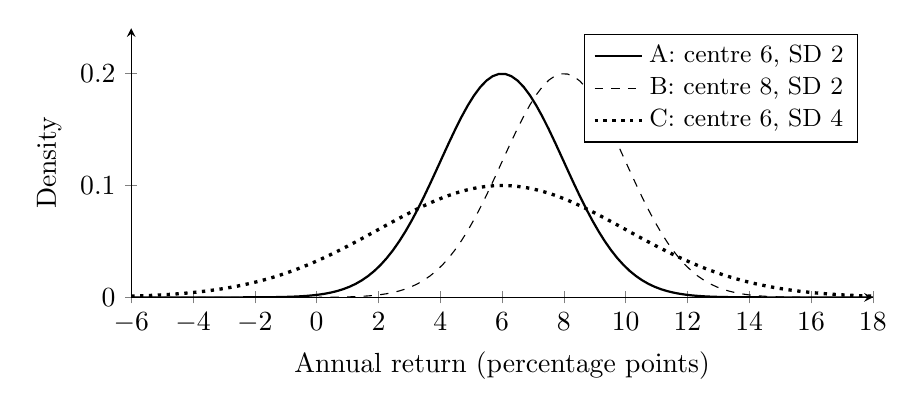
\begin{tikzpicture}
\begin{axis}[width=11cm,height=5cm,axis lines=left,xlabel={Annual return (percentage points)},ylabel={Density},xmin=-6,xmax=18,ymin=0,ymax=.24,legend style={at={(.98,.98)},anchor=north east,font=\small}]
\addplot[black,thick,domain=-6:18,samples=120]{exp(-((x-6)^2)/8)/(2*sqrt(2*pi))};\addlegendentry{A: centre 6, SD 2}
\addplot[black,dashed,domain=-6:18,samples=120]{exp(-((x-8)^2)/8)/(2*sqrt(2*pi))};\addlegendentry{B: centre 8, SD 2}
\addplot[black,dotted,very thick,domain=-6:18,samples=120]{exp(-((x-6)^2)/32)/(4*sqrt(2*pi))};\addlegendentry{C: centre 6, SD 4}
\end{axis}\end{tikzpicture}\end{center}
B is a two-percentage-point right shift of A, with equal spread and peak height. C has A's mean but twice the SD and four times the variance. Its curve is wider and its peak lower, preserving area one. For this normal family, more probability lies farther than any fixed positive distance from the shared mean in C than in A. This is a statement about spread, not a larger expected return.
\secInicio[prob:sec:general-worked1][sec:general-worked]


\subsection{Adding a fixed charge and changing the unit}\label{prob:sec:general-worked2}
Let an invoice charge $X$ in dollars have $E[X]=10$ dollars and $\operatorname{Var}(X)=4$ dollars squared. Define $Y=X+3$ dollars, and let $C=100X$ express the original charge in cents.
\QuestionsTasks[sec:general-worked]{{8}/{sol:sec:general-worked2}/{Find each transformed mean, variance and standard deviation. Explain the different graphical effects of adding a charge and changing measurement units.}}
\subsubsection*{Worked solution}\label{sol:sec:general-worked2}
Adding the fixed three-dollar charge shifts every observation equally:
\[
E[Y]=10+3=\HLPopulationMean{13}\text{ dollars},\quad
\operatorname{Var}(Y)=\HLPopulationVariance{4}\text{ dollars squared},\quad
\sigma_Y=2\text{ dollars}.
\]
Distances from the new mean are unchanged. Changing to cents rescales every horizontal distance:
\[
E[C]=100(10)=1000\text{ cents},\quad
\operatorname{Var}(C)=100^2(4)=40{,}000\text{ cents squared},
\]
\[
\sigma_C=\sqrt{40{,}000}=200\text{ cents}.
\]
The larger numerical variance in cents does not indicate greater underlying economic uncertainty: 200 cents is the same SD as two dollars. A density graph in cents is wider numerically and correspondingly lower so area stays one.
\secInicio[prob:sec:general-worked2][sec:general-worked]
\section{Advanced Problems}\label{sec:advanced}
\SectionProblemsTableOfContents{
\SectionProblemLink{prob:sec:advanced0}{Equal support and centre, different concentration}}

\subsection{Equal support and centre, different concentration}\label{prob:sec:advanced0}
Two forecast models describe a one-day handling cost in dollars. Model U is uniform on $[0,12]$. Model T is symmetric triangular through $(0,0),(6,1/6),(12,0)$. Use the supplied triangular variance formula.
\QuestionsTasks[sec:advanced]{{8}/{sol:sec:advanced0}/{Compare means, variances and the probabilities of costs from three to nine dollars. Explain how graph concentration supports the spread comparison.}}
\subsubsection*{Worked solution}\label{sol:sec:advanced0}
Both are symmetric around $\HLPopulationMean{6}$ dollars. Their variances are
\[
\sigma_U^2=12^2/12=\HLPopulationVariance{12},\qquad
\sigma_T^2=12^2/24=\HLPopulationVariance{6}
\]
in dollars squared. The uniform interval probability is $6/12=1/2$. For T, heights at three and nine are $1/12$; remove the two outer triangles:
\[
P_T(3<X<9)=1-2\left[\tfrac12(3)(1/12)\right]=\HLProbability{3/4}.
\]
The triangular model puts $75\%$ in the central band, compared with $50\%$ for U. It concentrates more area near the common mean and has lower variance. Equal endpoints do not force equal spread.
\PracticeDensity{-1}{13}{0.20}{0,3,6,9,12}{0,3,6,9,12}{0,0.083333,0.166667}{x}{0,$1/12$,$1/6$}{(0,0) (6,0.166667) (12,0)}
The triangular mean lies at the symmetry centre; its higher central peak is consistent with greater central concentration for this comparison, but a peak height by itself does not define variance.
\secInicio[prob:sec:advanced0][sec:advanced]

\end{document}

